\documentclass[10pt]{article}
\usepackage[a4paper, top=0.5in, bottom=0.5in, left=0.65in, right=0.65in]{geometry}
\usepackage{fontspec}
\usepackage[fontset=none]{ctex}
\setCJKmainfont{Noto Serif CJK SC}[BoldFont={Noto Serif CJK SC Bold}]
\usepackage{xcolor}
\usepackage{graphicx}
\usepackage{hyperref}
\usepackage{enumitem}
\usepackage{titlesec}
\usepackage{microtype}

\definecolor{linkblue}{HTML}{145A8D}
\hypersetup{
  colorlinks=true,
  urlcolor=linkblue,
  linkcolor=linkblue,
  citecolor=linkblue,
  breaklinks=true,
  unicode=true,
  pdftitle={周禧彬 - 中文简历},
  pdfauthor={周禧彬（Xibin Zhou）},
  pdflang={zh-CN}
}
\urlstyle{same}
\pagestyle{empty}
% Keep the Chinese CV on one A4 page with a readable 10 pt body.
\linespread{1.15}
\setlength{\parindent}{0pt}
\setlength{\parskip}{0pt}
\IfFontExistsTF{Times New Roman}{%
  \setmainfont{Times New Roman}%
}{%
  \setmainfont{TeX Gyre Termes}%
}
\titleformat{\section}{\large\bfseries}{}{0pt}{}
\titlespacing*{\section}{0pt}{6pt}{3pt}
\setlist[itemize]{nosep, leftmargin=*}

\begin{document}

% Keep the portrait and contact links consistent with the English CV.
\noindent
\begin{minipage}[c]{24mm}
  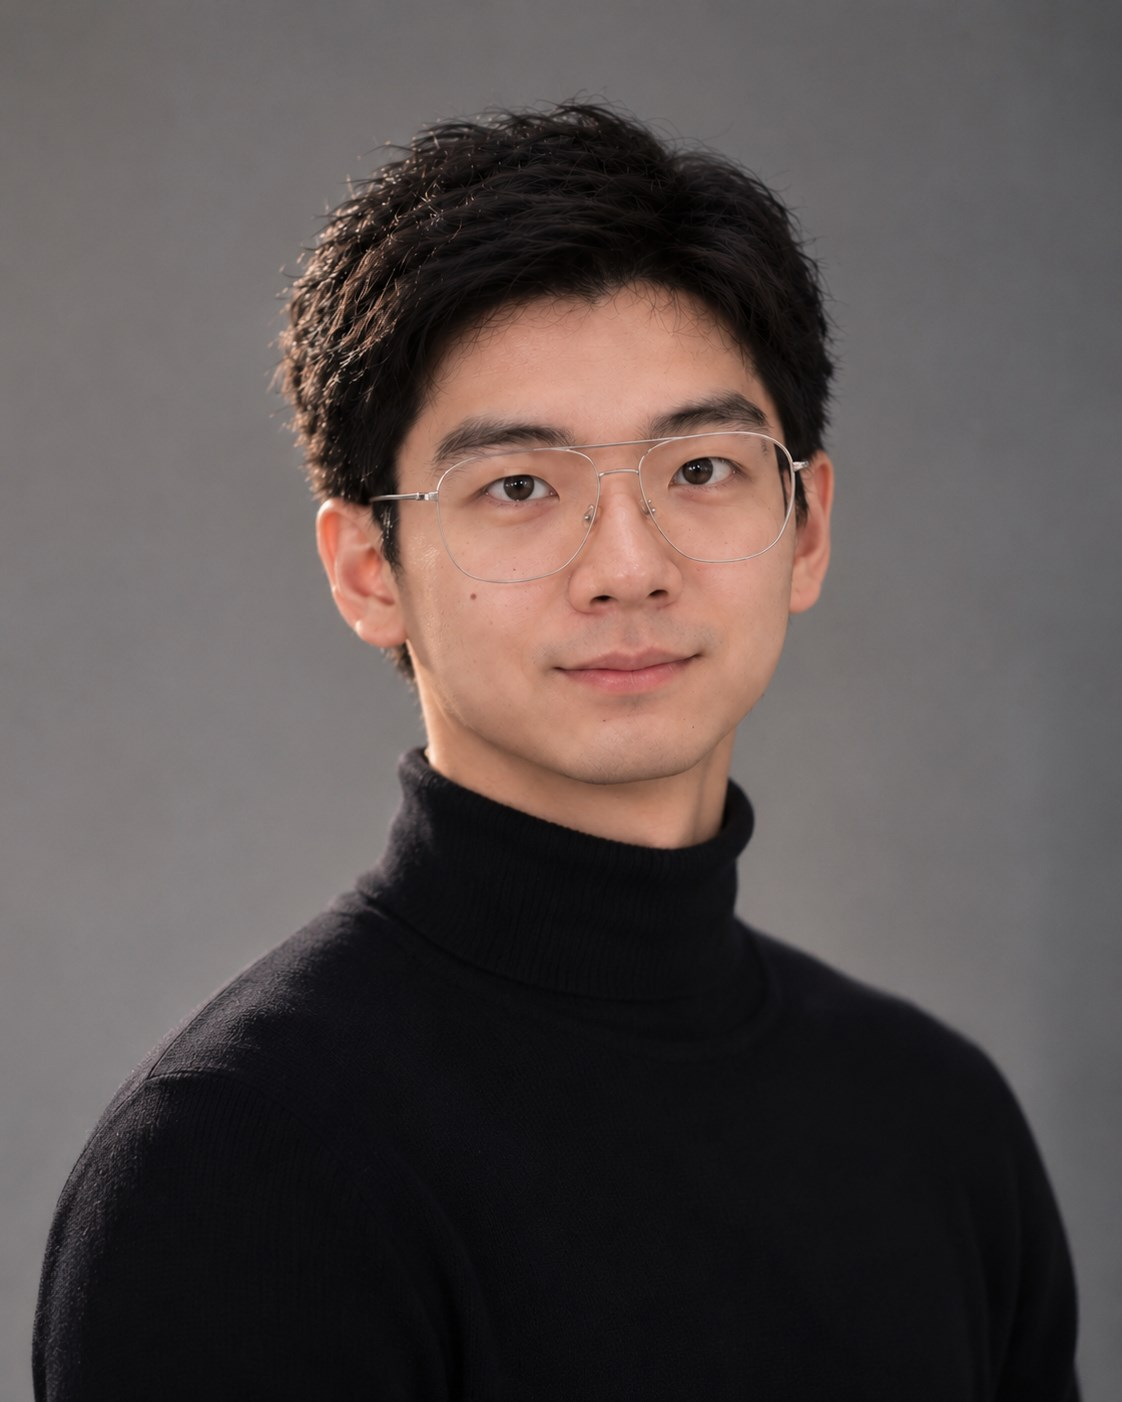
\includegraphics[width=\linewidth]{../../images/周禧彬-银框眼镜男士肖像-小.jpg}
\end{minipage}\hspace{6mm}%
\begin{minipage}[c]{\dimexpr\linewidth-30mm\relax}
\raggedright
{\Large \textbf{周禧彬（Xibin Bayes Zhou）}}\\[0.08cm]
面向检索、对话与设计的蛋白质基础模型\\[0.04cm]
西湖大学计算机科学博士生（与浙江大学联合培养）\enspace\textbar\enspace 杭州\\[0.04cm]
\href{https://zhoubay.github.io}{zhoubay.github.io} \textbar\
\href{mailto:zhouxibin@westlake.edu.cn}{zhouxibin@westlake.edu.cn} \textbar\
\href{https://scholar.google.com/citations?user=ey4rxTIAAAAJ}{Google Scholar} \textbar\
\href{https://orcid.org/0009-0007-8879-4966}{ORCID} \textbar\
\href{https://github.com/zhoubay}{GitHub} \textbar\
\href{https://www.linkedin.com/in/xibinbayeszhou/}{LinkedIn}
\end{minipage}\par
\vspace{4pt}

\section*{教育背景}
\begin{itemize}
    \item \textbf{西湖大学、浙江大学}，计算机科学博士研究生（联合培养），杭州 \hfill 2022--2027（预计）
    \item \textbf{同济大学}，数据科学与大数据技术，工学学士，上海 \hfill 2018--2022
    \item \textbf{天津南开中学}，高中，天津 \hfill 2015--2018
\end{itemize}

\section*{研究方向}
\begin{itemize}
    \item \textbf{结构感知蛋白质语言模型}：融合三维结构词元与序列，构建通用蛋白质语言模型。
    \item \textbf{多模态蛋白质理解}：对齐序列、结构与自然语言，支持蛋白质检索与功能注释。
    \item \textbf{AI 驱动的蛋白质工程}：酶优化、碱基编辑、从头设计与自主实验流程。
    \item \textbf{降低蛋白质语言模型研究门槛}：面向生物学研究者的无代码训练平台与开放协作。
\end{itemize}

\section*{荣誉奖励}
\begin{itemize}
    \item \textbf{2025 年 10 月} --- \textbf{最佳海报奖}，\textit{Nature Conference on AI Augmented Biology}（南京；Evolla 研究海报）
\end{itemize}

\section*{开源贡献与科研传播}
\begin{itemize}
    \item Hugging Face \textbf{Transformers 贡献者}：参与 Evolla 集成 --- \href{https://github.com/huggingface/transformers/commit/45c7bfb1571160d2c06b880073a5c73e6bfa3677}{代码提交}
    \item \textbf{Evolla} 在 X 平台的介绍帖浏览量超 \textbf{13 万} --- \href{https://x.com/duguyuan/status/1876446845951492221}{帖子}
    \item \textbf{Evolla} 在 Hugging Face 的累计下载量超 \textbf{100 万} --- \href{https://huggingface.co/westlake-repl/Evolla-10B-hf}{模型} \textbar\ \href{https://huggingface.co/api/models/westlake-repl/Evolla-10B-hf?expand\%5B\%5D=downloadsAllTime}{验证（API）}
    \item \textbf{Pinal} 获 \textit{Nature News} 报道（2025 年 5 月）--- \href{https://www.nature.com/articles/d41586-025-01586-y}{报道}
    \item \textbf{Pinal} 研究获\textbf{西湖大学}新闻报道（2026 年 10 月）--- \href{https://www.westlake.edu.cn/news_events/westlakenews/Research/202610/t20261022_70597.html}{报道} \textbar\ \href{https://zhoubay.github.io/files/evidence/westlake-press-pinal.png}{照片}
    \item \textbf{ProTrek} 研究获\textbf{西湖大学}新闻报道（2025 年 10 月）--- \href{https://www.westlake.edu.cn/news_events/westlakenews/Research/202510/t20251030_60873.html}{报道} \textbar\ \href{https://zhoubay.github.io/files/evidence/westlake-press.jpg}{照片}
\end{itemize}

% Retain original titles, author order, venues, and links for discoverability.
\section*{代表性论文}
{\footnotesize * 表示共同贡献}
\begin{itemize}
    \item \textbf{Xibin Zhou}, \textit{et al.} \href{https://doi.org/10.1101/2025.01.05.630192}{\textbf{Decoding the molecular language of proteins with Evolla}}. \textit{bioRxiv}（\textit{Nature} 审稿中）, 2025.
    \item F. Dai, \textit{et al.}, \textbf{X. Zhou}. \href{https://doi.org/10.1038/s41586-026-11205-z}{\textbf{Programmable design of functional proteins from natural language}}. \textit{Nature}, 2026. DOI: \href{https://doi.org/10.1038/s41586-026-11205-z}{10.1038/s41586-026-11205-z}
    \item Y. He*, \textbf{X. Zhou*}, \textit{et al.} \href{https://doi.org/10.1016/j.molcel.2024.01.021}{\textbf{PLM-assisted optimization of uracil-N-glycosylase enables programmable T-to-G/C base editing}}. \textit{Molecular Cell} 84(7), 1257--1270, 2024.
    \item H. Qian*, Y. Wang*, \textbf{X. Zhou*}, \textit{et al.} \href{https://doi.org/10.1038/s41467-025-58521-y}{\textbf{ESM-Ezy: deep learning strategy for mining novel multicopper oxidases}}. \textit{Nature Communications} 16, 3274, 2025.
    \item J. Su*, Y. He*, S. You*, \textit{et al.}, \textbf{X. Zhou}. \href{https://doi.org/10.1038/s41587-025-02836-0}{\textbf{A trimodal protein language model enables advanced protein searches}}. \textit{Nature Biotechnology}, 2025.
    \item J. Su, \textit{et al.}, \textbf{X. Zhou}. \href{https://doi.org/10.1038/s41587-025-02859-7}{\textbf{Democratizing protein language model training, sharing and collaboration}}. \textit{Nature Biotechnology}, 2025.
    \item J. Su, \textit{et al.}, \textbf{X. Zhou}. \href{https://openreview.net/forum?id=6MRm3G4NiU}{\textbf{SaProt: protein language modeling with structure-aware vocabulary}}. \textit{ICLR}, 2024.
\end{itemize}

\section*{实习经历}
\begin{itemize}
    \item \textbf{真格基金}，投资实习生 \hfill 2023 年 7--9 月（远程）
\end{itemize}

\section*{课外活动}
\begin{itemize}
    \item 西湖大学水上运动俱乐部\textbf{前会长}；\textbf{赛艇}（4 年，队长）；\textbf{桨板}（3 年）；帆船、龙舟及桨板球。
\end{itemize}

\section*{体育荣誉}
\begin{itemize}
    \item \textbf{2026 年 10 月 18 日} --- \textbf{全国高校组第三名}，2026 年中国桨板球公开赛上海站；\\
    代表西湖大学水上运动俱乐部首发参赛。
\end{itemize}

\section*{语言能力}
\begin{itemize}
    \item 普通话（母语；普通话水平测试一级乙等）、英语（熟练）、日语（JLPT N2）
    \item 西班牙语、拉丁语（学习中）
\end{itemize}

\end{document}
